\let\negmedspace\undefined
\let\negthickspace\undefined
\documentclass[journal]{IEEEtran}
\usepackage[a5paper, margin=10mm, onecolumn]{geometry}
%\usepackage{lmodern} % Ensure lmodern is loaded for pdflatex
\usepackage{tfrupee} % Include tfrupee package

\setlength{\headheight}{1cm} % Set the height of the header box
\setlength{\headsep}{0mm}     % Set the distance between the header box and the top of the text
\usepackage{xparse}
\usepackage{gvv-book}
\usepackage{gvv}
\usepackage{cite}
\usepackage{amsmath,amssymb,amsfonts,amsthm}
\usepackage{algorithmic}
\usepackage{graphicx}
\usepackage{textcomp}
\usepackage{xcolor}
\usepackage{txfonts}
\usepackage{listings}
\usepackage{enumitem}
\usepackage{mathtools}
\usepackage{gensymb}
\usepackage{comment}
\usepackage[breaklinks=true]{hyperref}
\usepackage{tkz-euclide} 
\usepackage{listings}
% \usepackage{gvv}                                        
\def\inputGnumericTable{} 
\usepackage[latin1]{inputenc}                                
\usepackage{color}                                            
\usepackage{array}                                            
\usepackage{longtable}                                       
\usepackage{calc}                                             
\usepackage{multirow}                                         
\usepackage{hhline}                                           
\usepackage{ifthen}                                           
\usepackage{lscape}

\begin{document}

\bibliographystyle{IEEEtran}
\vspace{3cm}

\title{9-9.3-27}
\author{EE24BTECH11006 - Arnav Mahishi}
% \maketitle
% \newpage
% \bigskip
{\let\newpage\relax\maketitle}

\renewcommand{\thefigure}{\theenumi}
\renewcommand{\thetable}{\theenumi}
\setlength{\intextsep}{10pt} % Space between text and floats


\numberwithin{equation}{enumi}
\numberwithin{figure}{enumi}
\renewcommand{\thetable}{\theenumi}
Question: Using Integration, find the area of the smaller region bounded by the ellipse $\frac{x^2}{9}+\frac{y^2}{4}=1$ and the line $\frac{x}{3}+\frac{y}{2}=1$\\
\begin{table}[h!]    
  \centering
  \begin{table}[H]
    \centering
    \begin{tabular}{|c|c|c|c|c|c|c|}
        \hline
        & \multicolumn{4}{c|}{\textbf{DESTINATIONS}} & \textbf{Supply} \\ \cline{2-5}
        \textbf{SOURCES} & P & Q & R & S & \\ \hline
        \textbf{1} & 13 & 8 & 12 & 9 & 20 \\ \hline
        \textbf{2} & 10 & 7 & 5 & 20 & 10 \\ \hline
        \textbf{3} & 3 & 19 & 5 & 12 & 50 \\ \hline
        \textbf{4} & 4 & 9 & 7 & 15 & 30 \\ \hline
        \textbf{5} & 14 & 0 & 1 & 7 & 40 \\ \hline
        \textbf{Demand} & 60 & 10 & 20 & 60 & \\ \hline
    \end{tabular}
\end{table} 

  \caption{Input Parameters}
\end{table}\\
Solution:\\
The point of intersection of the line with the ellipse is $x_i=h+k_i m$,\\
where,$k_i$ is a constant and is calculated as follows:-
$$k_i=\frac{1}{m^\top Vm}\brak{-m^\top \brak{Vh+u}\pm \sqrt{\sbrak{m^\top \brak{Vh+u}}^2-g\brak{h}\brak{m^\top Vm}}}$$\\
Substituting the input parameters in $k_i$,\\
\begin{multline}
     k_i =\frac{1}{\myvec{\frac{1}{b}&\frac{-1}{a}}\myvec{b^2&0\\0&a^2}\myvec{\frac{1}{b}\\\frac{-1}{a}}}\brak{-\myvec{\frac{1}{b}&\frac{-1}{a}}\brak{\myvec{b^2&0\\0&a^2}\myvec{a\\0}+\myvec{0\\0}}\pm \\
     \sqrt{\sbrak{\myvec{\frac{1}{b}&\frac{-1}{a}}\brak{\myvec{b^2&0\\0&a^2}\myvec{a\\0}+\myvec{0\\0}}}^2-g\brak{h}\brak{\myvec{\frac{1}{b}&\frac{-1}{a}}\myvec{b^2&0\\0&a^2}\myvec{\frac{1}{b}\\\frac{-1}{a}}}}} 
\end{multline}
We get,\\
$$k_i= 0,-ab$$
Substituting $k_i$ in $x_i=h+k_i m$  we get,\\
\begin{align}
     x_1&=\myvec{a\\0}+\brak{0}\myvec{\frac{1}{b}\\\frac{-1}{a}}\\
    \implies x_1 &=\myvec{a\\0}\\
    x_2 &=\myvec{a\\0}+\brak{-ab}\myvec{\frac{1}{b}\\\frac{-1}{a}}\\
    \implies x_2&=\myvec{a\\0}+\myvec{-a\\b}\\
    \implies x_2&=\myvec{0\\b}
\end{align}
The area of the smaller region bounded by the ellipse $\frac{x^2}{9}+\frac{y^2}{4}=1$ and the line $\frac{x}{3}+\frac{y}{2}=1$ is
\begin{align}
    &=\int_{0}^{a} \frac{b}{a}\sqrt{a^2-x^2} \,dx-\int_{0}^{a} \frac{b}{a}\brak{a-x} \,dx\\
    &=\frac{b}{a}\brak{\frac{x}{2}\sqrt{a^2-x^2}+\frac{a^2}{2}\sin^{-1}{\frac{x}{a}}-ax+\frac{x^2}{2}}\limits_{0}^{a}\\
    &=\frac{b}{a}\brak{\frac{\pi a^2}{4}-\frac{a^2}{2}}=\frac{ab}{2}\brak{\frac{\pi}{2}-1}
\end{align}
The given area is $\frac{ab}{2}\brak{\frac{\pi}{2}-1}$ sq. units\\
$\therefore$ Upon substituting $a=3,b=2$ the given area is $3\brak{\frac{\pi}{2}-1}\text{sq. units}\approx1.712$ sq. units\\
\begin{figure}[h!]
   \centering
   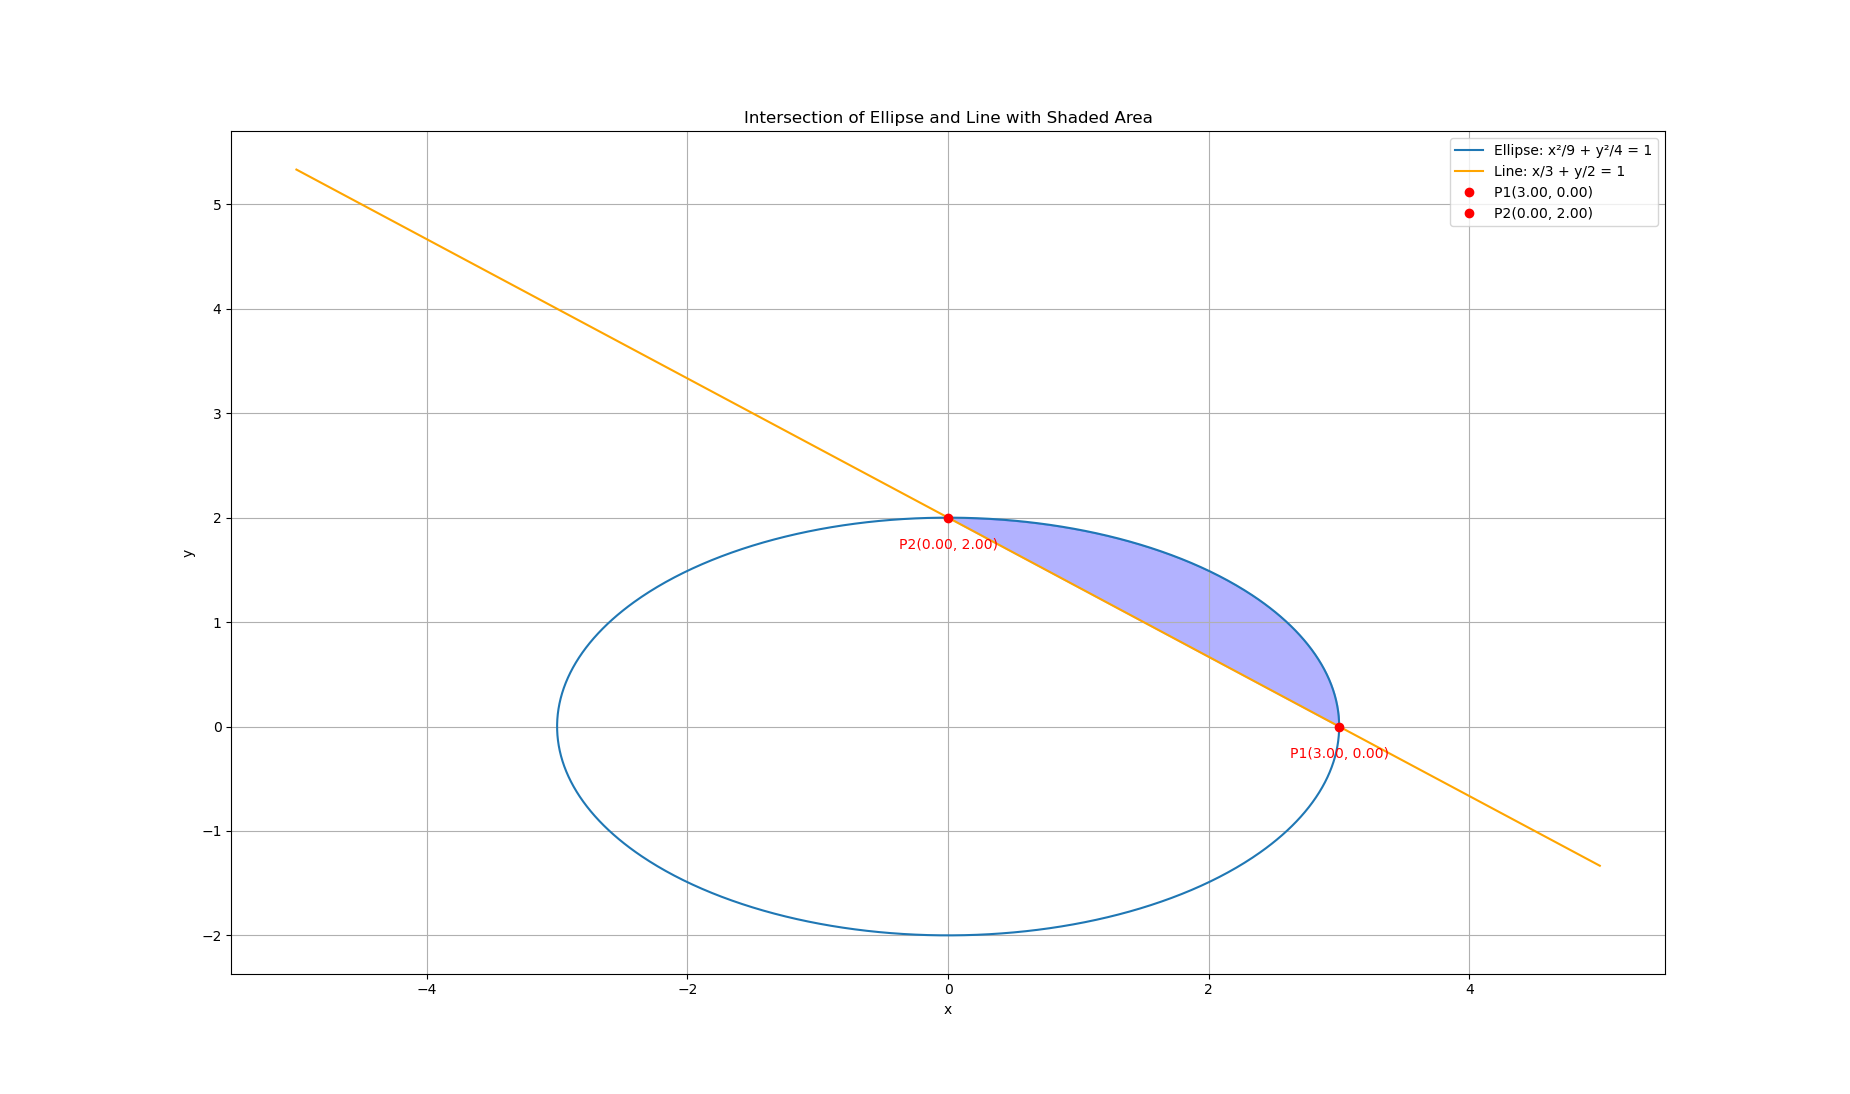
\includegraphics[width=0.7\linewidth]{figs/Figure_1.png}
   \caption{Plot of Ellipse and Line}
   \label{stemplot}
\end{figure}
\end{document}

